% Author Alfredo Sánchez Alberca (asalber@ceu.es)

\newproblem{pro-1}{far}{}
%ENUNCIADO
{En una estantería en la que hay 3 cajas de un medicamento $A$ y 2 de un medicamento $B$, se eligen 3 al azar.
¿Cuál es la probabilidad de que se hayan elegido 2 cajas del medicamento $A$ y 1 del $B$?
}
%SOLUCIÓN
{$36/60$.}
%RESOLUCIÓN
{}


\newproblem{pro-2}{far}{}
%ENUNCIADO
{En un laboratorio hay 4 frascos de ácido sulfúrico y 2 de ácido nítrico, y en otro hay 1 frascos de ácido sulfúrico y
3 de ácido nítrico.
Se saca al azar un frasco de cada laboratorio. Hallar la probabilidad de que:

\begin{enumerate}
\item  Los dos frascos sean de ácido sulfúrico.
\item  Los dos sean de ácido nítrico.
\item  Uno sea de ácido sulfúrico y otro de ácido nítrico.
\item Calcular la probabilidad de estos mismos sucesos si el frasco elegido en el primer laboratorio se introduce en el
segundo antes de sacar el frasco de este. 
\end{enumerate}
}
%SOLUCIÓN
{
\begin{enumerate}
\item $4/24$.
\item $6/24$.
\item $14/24$.
\item $8/30$, $8/30$ y $14/30$ respectivamente. 
\end{enumerate}
}
%RESOLUCIÓN
{}


\newproblem{pro-3}{gen}{}
%ENUNCIADO
{Sean $A$ y $B$ sucesos de un mismo espacio muestral tales que: $P(A)=3/8$, $P(B)=1/2$, $P(A\cap B)=1/4$.

Calcular:
\begin{enumerate}
\item  $P(A\cup B)$.
\item  $P(\overline{A})$ y $P(\overline{B})$.
\item  $P(\overline{A}\cap \overline{B})$.
\item  $P(A\cap \overline{B})$.
\item  $P(A/B)$.
\item  $P(A/\overline{B})$.
\end{enumerate}
}
%SOLUCIÓN
{
\begin{enumerate}
\item  $P(A\cup B)=5/8$.
\item  $P(\overline{A})=5/8$ y $P(\overline{B})=1/2$.
\item  $P(\overline{A}\cap \overline{B})=3/8$.
\item  $P(A\cap \overline{B})=1/8$.
\item  $P(A/B)=1/2$.
\item  $P(A/\overline{B})=1/4$.
\end{enumerate}
}
%RESOLUCIÓN
{}


\newproblem*{pro-4}{gen}{}
%ENUNCIADO
{Dado el siguiente circuito
\[
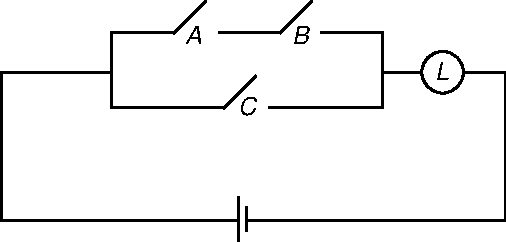
\includegraphics[scale=0.6]{img/circuito-pro-4}
 \]
si la probabilidad de estar cerrado el interruptor $A$ es $0.8$, el $B$ $0.9$ y el $C$ $0.7$, ¿cuál es la probabilidad
de que esté encendida la lámpara $L$?
}
%SOLUCIÓN
{}
%RESOLUCIÓN
{}


\newproblem{pro-5}{med}{}
%ENUNCIADO
{La probabilidad de contraer hepatitis a partir de una unidad de sangre es 0'01. Un paciente recibe dos unidades de
sangre durante su estancia en el hospital.
¿Cuál es la probabilidad de que contraiga hepatitis como consecuencia de ello?}
%SOLUCIÓN
{$0.0199$.}
%RESOLUCIÓN
{}


\newproblem*{pro-6}{far}{}
%ENUNCIADO
{En un lapso de tiempo una ameba puede morir con probabilidad 1/4 y dividirse en dos con probabilidad 1/2.
Durante el siguiente lapso de igual duración con cada ameba, independientemente de su origen, ocurre lo mismo.
¿Cuántas amebas y con qué probabilidad pueden existir al final del segundo intervalo de tiempo?
}
%SOLUCIÓN
{}
%RESOLUCIÓN
{}


\newproblem*{pro-7}{gen}{*}
%ENUNCIADO
{Supongamos los sucesos independientes $A_{1}$ y $A_{2}$ con probabilidades $p_{1}$ y $p_{2}$ respectivamente, e
incompatibles ambos con el suceso $A_{3}$ con probabilidad $p_{3}$ ($A_{1}$, $A_{2}$ y $A_{3}$ son sucesos de un mismo
espacio muestral).
Calcular en función de $p_{1}$, $p_{2}$ y $p_{3}$ las probabilidades de los siguientes sucesos:
\begin{enumerate}
\item  $A_{1}-(A_{2}\cup A_{3})$.
\item  $\overline{A_{1}\cup A_{2}\cup A_{3}}$.
\item  $A_{1}/(A_{2}\cup A_{3})$.
\end{enumerate}
}
%SOLUCIÓN
{}
%RESOLUCIÓN
{}


\newproblem{pro-8}{gen}{}
%ENUNCIADO
{Sean $A$ y $B$ sucesos de un mismo espacio muestral, tales que $P(A)=0.6$ y $P(A\cup B)=0.9$.
Calcular $P(B)$ si:
\begin{enumerate}
\item  $A$ y $B$ son incompatibles.
\item  $A$ y $B$ son independientes.
\end{enumerate}
}
%SOLUCIÓN
{
\begin{enumerate}
\item $P(B)=0.3$.
\item $P(B)=0.75$.
\end{enumerate}
}
%RESOLUCIÓN
{}


\newproblem{pro-9}{med}{*}
%ENUNCIADO
{En un estudio sobre el tabaco, se informa que el 40\% de los fumadores tiene un padre fumador, el 25\% tiene una madre
fumadora, y el 52\% tiene al menos uno de los dos padres fumadores. Se elige una persona fumadora al azar.
Calcular:
\begin{enumerate}
\item Probabilidad de que la madre sea fumadora si lo es el padre.
\item Probabilidad de que la madre sea fumadora si no lo es el padre.
\item ¿Son independientes el tener padre fumador y el tener madre fumadora?
\end{enumerate}
}
%SOLUCIÓN
{Llamando $PF$ al suceso que consiste en tener un padre fumador y $MF$ a tener una madre fumadora:
\begin{enumerate}
\item $P(MF/PF)=0.325$.
\item $P(MF/\overline{PF})=0.2$.
\item No son independientes.
\end{enumerate}
}
%RESOLUCIÓN
{Llamando $PF$ al suceso que consiste en tener un padre fumador y $MF$ a tener una madre fumadora, del enunciado se
tiene que $P(PF)=0.4$, $P(MF)=0.25$ y $P(PF\cup MF)=0.52$.
\begin{enumerate}
\item Nos piden la probabilidad de tener madre fumadora condicionada por tener padre fumador. Según la definción de
probabilidad condicionada se tiene
\[
P(MF/PF) = \frac{P(MF\cap PF)}{P(PF)}.
\]
A su vez, la probabilidad de la intersección de tener madre y padre fumadores puede calcularse a partir de la fórmula
de la unión:
\[
P(MF\cup PF) = P(MF)+P(PF)-P(MF\cap PF) \Leftrightarrow P(MF\cap PF) = P(MF)+P(PF)-P(MF\cup PF) = 0.4+0.25-0.52= 0.13,
\]
de modo que la probabilidad condicionada queda
\[
P(MF/PF) = \frac{P(MF\cap PF)}{P(PF)} = \frac{0.13}{0.4}=0.33.
\]
\item Ahora nos piden la probabilidad de tener madre fumadora condicionada por tener padre no fumador. De nuevo, según
la definición de probabilidad condicionada se tiene
\[
P(MF/\overline{PF}) = \frac{P(MF\cap \overline{PF})}{P(\overline{PF})}.
\]
Como el suceso $MF\cap \overline{PF}$ es la diferencias del suceso $MF$ y el suceso $PF$, su probabilidad se puede
calcular como
\[
P(MF\cap \overline{PF}) = P(MF)-P(MF\cap PF) = 0.25-0.13 = 0.12,
\]
de modo que la probabilidad condicionada queda
\[
P(MF/\overline{PF}) = \frac{P(MF\cap \overline{PF})}{P(\overline{PF})} = \frac{0.12}{1-0.4}=0.2.
\]
\item Como $P(MF)=0.25\neq 0.33=P(MF/PF)$ se puede concluir que los sucesos no son independientes. 
\end{enumerate}
}


\newproblem{pro-10}{med}{}
%ENUNCIADO
{El tétanos es mortal en el 70\% de los casos.
Si tres personas contraen el tétanos, ¿Cuál es la probabilidad de que mueran al menos dos de los tres?
}
%SOLUCIÓN
{$0.784$.}
%RESOLUCIÓN
{}


\newproblem{pro-11}{med}{*}
%ENUNCIADO
{Un equipo de atención primaria de salud realiza un estudio de la población, para evaluar la incidencia de hipertensión
e hipercolesterolemia.
Para ello analizan a 1000 personas de dicha población, seleccionadas aleatoriamente, encontrándose que 180 presentan
hipertensión, 140 hipercolesterolemia y 800 ninguna de ambas.
Se pide calcular la probabilidad de que una persona tomada al azar.
\begin{enumerate}
\item  Presente ambas enfermedades.
\item  Presente hipertensión si no presenta hipercolesterolemia.
\end{enumerate}
}
%SOLUCIÓN
{Llamando $HT$ a tener hipertensión y $HC$ a tener hipercolesterolemia:
\begin{enumerate}
\item $P(HT\cap HC)=0.12.$
\item $P(HT/\overline{HC})=0.0698.$
\end{enumerate} 
}
%RESOLUCIÓN
{}


\newproblem{pro-12}{gen}{*}
%ENUNCIADO
{Tras observar los resultados de la prueba de selectividad se sabe que el 40\% de los alumnos aprueba el examen de
Matemáticas, el 30\% el examen de Física y el 55\% suspenden los dos.
Si se elige un alumno al azar, calcular:
\begin{enumerate}
\item Probabilidad de que haya aprobado al menos uno de los dos exámenes.
\item Probabilidad de que haya aprobado Matemáticas si ha aprobado Física.
\item Probabilidad de que haya aprobado Física si ha suspendido Matemáticas.
\item ¿Son independientes aprobar Matemáticas y aprobar Física?
\end{enumerate}
}
%SOLUCIÓN
{Llamando $M$ al suceso correspondiente a aprobar Matemáticas y $F$ a aprobar Física:
\begin{enumerate}
\item $P(M\cup F)=0.45$.
\item $P(M/F)=0.83$.
\item $P(F/\overline{M})=0.08$.
\item No son independientes.
\end{enumerate}
}
%RESOLUCIÓN
{}


\newproblem{pro-13}{fis}{*}
%ENUNCIADO
{La probabilidad de que una lesión $A$ se reproduzca es $4/5$, la de que se reproduzca otra lesión $B$ es $1/2$, y la de que ambas se
reproduzcan $1/3$. Hallar la probabilidad de que:
\begin{enumerate}
\item Sólo se reproduzca la lesión $B$.
\item Al menos una se reproduzca.
\item Se reproduzca la lesión $B$ si se ha reproducido la $A$.
\item Se reproduzca la lesión $B$ si no se reproduce la lesión $A$.
\end{enumerate}
}
%SOLUCIÓN
{Llamando $A$ y $B$ a los sucesos consistentes en que se reproduzcan las respectivas lesiones, se tiene:
\begin{enumerate}
\item $P(B\cap\overline{A})=1/6$.
\item $P(A\cup B)=29/30$.
\item $P(B/A)=5/12$.
\item $P(B/\overline{A})=5/6$.
\end{enumerate}
}
%RESOLUCIÓN
{Llamemos $A$ y $B$ a los sucesos consistentes en que se reproduzcan las respectivas lesiones. Según el enunciado tenemos
$P(A)=4/5$, $P(B)=1/2$ y $P(A\cap B)=1/3$.

\begin{enumerate}
\item Para que sólo se reproduzca la lesión $B$ debe cumplirse el suceso $B-A$, es decir $B\cap\overline{A}$.
\[P(B\cap\overline{A})=P(B)-P(A\cap B)=1/2-1/3=1/6.\]

\item Para que se reproduzca al menos una lesión debe cumplirse el suceso $A\cup B$.
\[P(A\cup B)=P(A)+P(B)-P(A\cap B)=4/5+1/2-1/3=29/30.\]

\item El suceso consistente en que se reproduzca la lesión $B$ si se ha reproducido la $A$ es $B/A$.
\[P(B/A)=\frac{P(A\cap B)}{P(A)}=\frac{1/3}{4/5}=5/12.\]

\item El suceso consistente en que se reproduzca la lesión $B$ si no se ha reproducido la $A$ es $B/\overline{A}$.
\[P(B/\overline{A})=\frac{P(\overline{A}\cap B)}{P(\overline{A})}=\frac{1/6}{1-4/5}=5/6.\]
\end{enumerate}
}


\newproblem*{pro-14}{med}{}
%ENUNCIADO
{A partir de una investigación realizada, se sabe que el 10\% de las personas de 50 años sufren un tipo particular de
artritis.
Se ha desarrollado un procedimiento para detectar esta enfermedad, y por las pruebas realizadas se observa que si se
aplica el procedimiento a individuos que padecen la enfermedad, da positivo en el 85\% de los casos, mientras que
si se aplica a individuos sanos, da positivo en el 4\% de los casos.
Se pide:
\begin{enumerate}
\item  Calcular la probabilidad de que realizado el procedimiento a una persona, el resultado sea positivo.
\item  Si el resultado de aplicar el procedimiento a una persona ha sido positivo, ¿Cuál es la probabilidad de que
padezca la enfermedad?
\end{enumerate}
}
%SOLUCIÓN
{}
%RESOLUCIÓN
{}


\newproblem{pro-15}{gen}{*}
%ENUNCIADO
{En un experimento aleatorio se pueden dar dos sucesos $A$ y $B$, y se sabe que $P(B)=0.4$, $P(A/B)=0.3$ y
$P(A/\overline{B})=0.2$.
Calcular las siguientes probabilidades:
\begin{enumerate}
\item $P(A)$.
\item $P(\overline{A}\cap \overline{B})$.
\item $P(\overline{A}\cup \overline{B})$.
\end{enumerate}
}
%SOLUCIÓN
{
\begin{enumerate}
\item $P(A)=0.24$.
\item $P(\overline{A}\cap \overline{B})=0.52$.
\item $P(\overline{A}\cup \overline{B})=0.88$.
\end{enumerate}
}
%RESOLUCIÓN
{}


\newproblem{pro-16}{med}{*}
%ENUNCIADO
{En un servicio clínico digestivo se sabe que, de cada 1000 pacientes con dolor de estómago, 700 presentan gastritis,
200 presentan úlcera y 100 presentan cáncer.
En el análisis de la sintomatología gástrica, se ha comprobado que las probabilidades de presentar vómitos son $0.3$ en
el caso de gastritis, $0.6$ en el caso de úlcera y $0.9$ en el caso de cáncer.
Llega un nuevo paciente con dolor de estómago que, además, presenta vómitos.
¿Qué diagnosticaríamos?}
%SOLUCIÓN
{Llamando $G$ a tener gastritis, $U$ a tener úlcera, $C$ a tener cáncer y $V$ a tener vómitos, $P(G/V)=0.5$,
$P(U/V)=0.286$ y $P(C/V)=0.214$, de modo que se diagnosticaría gastritis.}
%RESOLUCIÓN
{}


\newproblem{pro-17}{gen}{*} 
%ENUNCIADO
{Un estudiante se somete a un examen de tipo test en el que cada pregunta tiene 3 respuestas posibles.
El estudiante se sabe el 40\% de las preguntas, y el resto las contesta al azar.
Se elige al azar una pregunta.
¿Qué probabilidad hay de que no la supiera si la contestó correctamente?
}
%SOLUCIÓN
{$1/3$.}
%RESOLUCIÓN
{}


\newproblem*{pro-18}{med}{*}
%ENUNCIADO
{Un test diseñado para diagnosticar el cáncer de cuello uterino da resultado positivo en el 10\% de los casos en los
que no existe la enfermedad, y da negativo en el 5\% de los casos en los que sí que existe la enfermedad.

Se sabe que en una cierta población de mujeres, el 4\% padece dicha enfermedad.
Si una mujer elegida aleatoriamente se somete al test, y da positivo, ¿qué probabilidad hay de que padezca la
enfermedad?}
%SOLUCIÓN
{}
%RESOLUCIÓN
{}


\newproblem{pro-19}{med}{*}
%ENUNCIADO
{Se ha desarrollado un nuevo test diagnóstico para detectar el síndrome de Down en niños recién nacidos, con un
sensibilidad del 80\% y una especificidad del 90\%.
Si en una determinada población en la que hay un 1\% de recién nacidos con el síndrome, al aplicarle el test a un niño,
da positivo, ¿cuál es la probabilidad de que tenga el síndrome?
¿le diagnosticarías la enfermedad?
¿Cuál debería ser la especificidad mínima del test para diagnosticar el síndrome en el caso de dar positivo?

Nota: La \emph{sensibilidad} de un test diagnóstico es la proporción de personas con la enfermedad que tienen un
resultado positivo en el test, mientras que la \emph{especificidad} del test es la proporción de personas sin la
enfermedad que tienen un resultado negativo en el test.}
%SOLUCIÓN
{Llamando $S$ a tener el síndrome de Down y $+$ a que el test de positivo, $P(S/+)=0.0748$ y
$P(\overline{S}/+)=0.9252$, de modo que no se diagnosticaría el síndrome al ser más probable que no lo tenga.\\
La especificidad mínima para que el test diagnostique el síndrome es $P(-/\overline{S})=0.9919$.}
%RESOLUCIÓN
{}


\newproblem{pro-20}{med}{*}
%ENUNCIADO
{En un estudio se han probado tres tipos de tratamientos $A$, $B$ y $C$ contra una determinada enfermedad. De los
pacientes participantes en el estudio, el 50\% fueron tratados con el tratamiento $A$, el 30\% con el $B$ y el 20\% con
el $C$.
Posteriormente se observaron los pacientes que sanaron y los que tuvieron algún efecto secundario, según se
muestra en la siguiente tabla:
\[
\begin{array}{|c|c|c|c|}
\hline
\text{Tratamiento} & \text{Sanados} & \text{Con efectos secundarios} \\
\hline
A & 86\% & 12\% \\
\hline
B & 92\% & 14\% \\
\hline
C & 81\% &  6\% \\
\hline
\end{array}
\]
Se pide:
\begin{enumerate}
\item Si se selecciona un enfermo al azar, ¿cuál es la probabilidad de que haya sanado?
¿Y de que haya tenido algún efecto secundario? 
\item Si un enfermo ha sanado, ¿qué tratamiento es más probable que haya recibido?
¿Y si en vez de decirnos que ha sanado nos dicen que no ha tenido efectos secundarios?
\item Si en total hay un 8\% pacientes que no sanaron pero que tampoco tuvieron efectos secundarios, ¿cuál es la
probabilidad de que un enfermo se haya curado sin tener efectos secundarios?
\end{enumerate}
}
%SOLUCIÓN
{Llamado $S$ a sanar y $E$ a tener efectos secundarios:
\begin{enumerate}
\item $P(S)=0.868$ y $P(E)=0.114$.
\item $P(A/S)=0.495$, $P(B/S)=0.318$ y $P(C/S)=0.187$.\\
$P(A/\overline{E})=0.497$, $P(B/\overline{E})=0.291$ y $P(C/\overline{E})=0.212$.\\
En ambos casos el tratamiento más probable es el $A$.
\item $P(S\cap \overline{E})=0.806$.
\end{enumerate}
}
%RESOLUCIÓN
{}


\newproblem*{pro-21}{nut}{}
%ENUNCIADO
{En una plantación hay tres variedades de uvas A,B y C en un 45\%, 35\% y 20\% respectivamente. Se sabe que el porcentaje de vides infectadas por una bacteria es del 5\% en la variedad A, del 12\% en la variedad B y del 18\% en la C. Si se toman uvas de una vid elegida al azar, ¿cuál es la probabilidad de que estén infectadas? Si las uvas cogidas de una vid están infectadas, ¿de qué variedad es más probable que sean?
}
%SOLUCIÓN
{}
%RESOLUCIÓN
{}


\newproblem*{pro-22}{amb}{}
%ENUNCIADO
{Se sabe que el 25\% de las plantas afectadas por un vertido tóxico están contaminadas. Se ha
desarrollado un procedimiento para detectar la contaminación, y por las
pruebas realizadas se observa que si se aplica el procedimiento a plantas contaminadas, da positivo en el 96\% de los casos, mientras que
si se aplica plantas no contaminadas, da positivo en el 8\% de los casos. Se pide:

\begin{enumerate}
\item  Calcular la probabilidad de que al aplicar el procedimiento a una planta elegida al azar, el resultado sea positivo.

\item  Si el resultado de aplicar el procedimiento a una planta ha sido
positivo, ¿Cuál es la probabilidad de que esté contaminada?
\end{enumerate}
}
%SOLUCIÓN
{}
%RESOLUCIÓN
{}


\newproblem*{pro-23}{amb}{}
%ENUNCIADO
{Un test para detectar la contaminación del agua tiene una sensibilidad del $97.5$\% y una especificidad del 95\%. Se pide:
\begin{enumerate}
\item ¿Qué relación existe entre la probabilidad de que el agua esté contaminada y la de que el test de positivo?
\item Si se aplica el test a muestras de 20 embalses y resulta positivo en 5 de las muestras, según la relación anterior, ¿qué porcentaje de embalses se estima que están contaminados?
\item Suponiendo que el porcentaje real de embalses contaminados es del 12\%, ¿cuál es la probabilidad de que un embalse esté contaminado si el resultado del test es negativo?
\end{enumerate}
}
%SOLUCIÓN
{}
%RESOLUCIÓN
{}


\newproblem*{pro-24}{med}{*}
% ENUNCIADO
{El dolor intenso sin derrame en una zona concreta de la articulación de la rodilla es síntoma de esguince en el Ligamento Lateral Externo
de la misma (L.L.E.). Si los esguinces en dicho ligamento se clasifican como: de grado 1, cuando hay simple distensión, que se presenta en
un 60\% de los casos; de grado 2, cuando hay ruptura parcial, que se presenta en un 30\% de los casos; y de grado 3, cuando hay ruptura
total, que se presenta en un 10\%. Y teniendo en cuenta que el síntoma se presenta en un 80\% de los que tienen el esguince de grado 1, en
un 90\% de los de grado 2, y en un 100\% de los de grado 3:
\begin{enumerate}
\item Si una persona se produce un esguince de L.L.E., ¿cuál es la probabilidad total de que padezca dolor intenso sin
derrame?
\item Si una persona llega a una consulta con dolor intenso sin derrame en la zona adecuada de la rodilla, ¿cuál sería
el diagnóstico?
\item De un total de 10000 personas analizadas con dolor intenso sin derrame en la zona adecuada de la rodilla,
¿cuántas se espera que hayan sufrido un esguince de grado 1?
¿Y de grado 2?
¿Y de grado3?
\item Si mantenemos iguales el resto de probabilidades dadas como dato, ¿cuáles deben ser las probabilidades de
esguince de grado 2 y de grado 3 para que la probabilidad de esguince de grado 2 si se padece el síntoma sea igual a la
de grado 3 si se padece el síntoma?
\end{enumerate}
}
%SOLUCIÓN
{}
%RESOLUCIÓN
{}


\newproblem{pro-25}{med}{*}
%ENUNCIADO
{En una población se ha vacunado a la tercera parte de los individuos contra la gripe.
Trascurrido el invierno, se comprueba que la probabilidad de estar vacunado si se tiene la gripe es $0.2$, y que el
10\% de los vacunados tuvieron gripe.
\begin{enumerate}
\item ¿Cuál fue la incidencia de la epidemia de gripe?\\
(Nota: La incidencia de una epidemia es la probabilidad de
personas infectadas).
\item ¿Cuál es la probabilidad de que una persona no vacunada contraiga la gripe?
\item ¿Se puede afirmar que la vacuna tiene alguna eficacia?
\end{enumerate}
}
%SOLUCIÓN
{Llamando $G$ al suceso consistente en tener la gripe y $V$ a estar vacunado:
\begin{enumerate}
\item $P(G)=1/6$.
\item $P(G/\overline{V})=0.2$.
\item Si resulta eficaz, aunque poco.
\end{enumerate}
}
%RESOLUCIÓN
{}


\newproblem*{pro-26}{amb}{*}
%ENUNCIADO
{Una zona de un Parque Nacional se ha repoblado con 10000
árboles, de los cuales 5000 han sido pinos, 4000 encinas y 1000
fresnos. Al cabo de un año se hace recuento y se observa que han
sobrevivido 4500 pinos, 2000 encinas y 900 fresnos. Suponiendo que
los resultados obtenidos son aplicables a una nueva zona del Parque
Nacional que se va a repoblar:
\begin{enumerate}
\item ¿Cuál es la probabilidad de que un árbol que se va a plantar
muera durante el primer año?
\item ¿Cuál es la probabilidad de que muera y sea pino?
\item Si sabemos que el árbol ha vivido, ¿cuál es la probabilidad de
que sea un fresno?
\item Si sabemos que el árbol ha muerto, ¿cuál es la probabilidad de
que sea una encina?
\end{enumerate}
}
%SOLUCIÓN
{}
%RESOLUCIÓN
{}


\newproblem*{pro-27}{gen}{}
%ENUNCIADO
{Sean $A$, $B$ y $C$ sucesos arbitrarios de un experimento
aleatorio. Se consideran los siguientes sucesos:
\begin{quote}
    $E_1$=\{al menos dos de los sucesos ocurren\},\\
    $E_2$=\{exactamente dos de los sucesos ocurren\},\\
    $E_3$=\{al menos uno de los sucesos ocurre\},\\
    $E_4$=\{exactamente uno de los sucesos ocurre\},\\
    $E_5$=\{no m\'{a}s de dos sucesos ocurren\}.
\end{quote}
Expresar $E_1$, $E_2$, $E_3$, $E_4$ y $E_5$ en función de $A$,$B$ y $C$.
}
%SOLUCIÓN
{}
%RESOLUCIÓN
{}


\newproblem*{pro-28}{gen}{}
%ENUNCIADO
{La probabilidad de que un hombre siga vivo dentro de 25 años es 3/5, y la de que su esposa lo esté es 2/3. Si
ambos sucesos son independientes, hallar la probabilidad de que en ese momento:
\begin{enumerate}
\item Ambos estén vivos.
\item Sólo el hombre viva.
\item Sólo viva la esposa.
\item Al menos uno esté vivo.
\item Viva el hombre si vive la esposa.
\item Viva el hombre si no vive la esposa.
\end{enumerate}
}
%SOLUCIÓN
{}
%RESOLUCIÓN
{}


\newproblem*{pro-29}{gen}{}
%ENUNCIADO
{La probabilidad de que un hombre siga vivo dentro de 25 años es 3/5, la de que su esposa lo esté es 2/3 y la de que
ambos vivan es 1/2. Hallar la probabilidad de que en ese momento:
\begin{enumerate}
\item Sólo el hombre viva.
\item Sólo viva la esposa.
\item Al menos uno esté vivo.
\item Viva el hombre si vive la esposa.
\item Viva el hombre si no vive la esposa.
\end{enumerate}
}
%SOLUCIÓN
{}
%RESOLUCIÓN
{}


\newproblem*{pro-30}{gen}{}
%ENUNCIADO
{El 40\% de los alumnos que han suspendido matemáticas deciden preparar el examen extraordinario en una academia, el
35\% decide asistir a las clases que organiza la propia universidad y el resto lo prepara por su cuenta.
De experiencias previas, se sabe que el 30\% de los alumnos de academia consigue aprobar el examen, de los alumnos que
asisten a la universidad aprueban el 45\%, y del resto de los alumnos aprueban el 25\%.
Se pide:
\begin{enumerate}
\item ¿Cuál es la probabilidad de que un alumno elegido al azar apruebe el examen?
\item Si un alumno ha suspendido, ¿cuál es la probabilidad de que haya asistido a una academia?
\end{enumerate}
}
%SOLUCIÓN
{}
%RESOLUCIÓN
{}


\newproblem*{pro-31}{gen}{}
%ENUNCIADO
{Se dispone de dos urnas, la primera con 10 bolas blancas y 6 bolas negras, y la segunda con 5 bolas rojas, 8 bolas
azules y 3 bolas verdes.
Construir el espacio muestral del experimento que consiste en sacar una bola de cada urna, y
del experimento que consistiría en sacar dos bolas de cada urna.}
%SOLUCIÓN
{}
%RESOLUCIÓN
{}


\newproblem*{pro-32}{amb}{}
%ENUNCIADO
{Una ciudad se abastece de agua de tres pantanos: $A$ en un 50\%, $B$ en un 40\% y $C$ en un 10\%. El agua del pantano $A$ produce diarrea en un 3\% de los casos, la del $B$ en un 1\% y la del $C$ en un $7\%$. ¿Cual es la probabilidad de que una persona que beba agua en la ciudad tenga diarrea? Si una persona presenta diarrea por causa del agua, ¿de qué pantano es más probable que provenga dicha agua?
}
%SOLUCIÓN
{}
%RESOLUCIÓN
{}

\newproblem*{pro-33}{gen}{}
%ENUNCIADO
{Construir el espacio muestral de los siguientes experimentos aleatorios:
\begin{enumerate}
\item Seleccionar una persona al azar y medir su sexo y si es fumadora o no. 
\item Seleccionar una persona al azar y medir su grupo sanguíneo y si es fumadora o no.
\item Seleccionar una persona al azar y medir su sexo, grupo sanguíneo y se es fumadora o no.
\end{enumerate}
}
%SOLUCIÓN
{}
%RESOLUCIÓN
{}


\newproblem*{pro-34}{amb}{*}
%ENUNCIADO
{Un test diagnóstico permite detectar la presencia de un tóxico en el pescado con una sensibilidad del 96\% y una especificidad del 92\%. Si un vertido ha afectado a las tres quintas partes del pescado de un lago, se pide:
\begin{enumerate}
\item ¿Cuál es la probabilidad de que al aplicar el test a un pescado  elegido al azar de negativo?
\item Si el test da negativo en un pescado, ¿es más probable que esté contaminado o que no lo esté?
\item ¿Podríamos decir lo mismo en un lago donde el 90\% de los pescados hayan sido contaminados?
\end{enumerate}
}
%SOLUCIÓN
{}
%RESOLUCIÓN
{}


\newproblem*{pro-35}{amb}{}
%ENUNCIADO
{Se han realizado tres campañas $A$, $B$ y $C$ de sensibilización para el reciclaje de vidrio y papel. La campaña $A$ se ha aplicado al 50\% de la población, la $B$ al 20\%, y al resto se la ha aplicado la $C$. Posteriormente se observaron las personas que acabaron reciclando habitualmente el vidrio y el papel, obteniendo los siguientes resultados
\begin{center}
\begin{tabular}{|c|c|c|}
\hline
$A$ & 56\% & 42\% \\
\hline
$B$ & 52\% & 46\% \\
\hline
$C$ & 71\% & 38\% \\
\hline
\end{tabular}
\end{center}
Se pide:
\begin{enumerate}
\item Si se selecciona un individuo al azar, ¿cuál es la probabilidad de que recicle vidrio? ¿Y de que recicle papel?
\item Si un individuo recicla vidrio, ¿qué campaña es más probable que haya recibido? ¿Y si en vez de decirnos que recicla vidrio nos dicen que recicla papel?
\item Si en total hay un 18\% de personas que no reciclan ni vidrio ni papel, ¿cuál es la probabilidad de que una persona recicle vidrio si no recicla papel?
\end{enumerate}
}
%SOLUCIÓN
{}
%RESOLUCIÓN
{}


\newproblem*{pro-36}{far}{*}
%ENUNCIADO
{Una enfermedad se trata con 3 fármacos diferentes, $A$, $B$ y $C$. El fármaco $A$ se aplica a un 30\% de los hombres y a un 50\% de las mujeres; el fármaco $B$ se aplica a un 60\% de los hombres y a un 20\% de las mujeres; y el fármaco $C$ a un 10\% de los hombres y al 30\% de las mujeres. Además, se sabe que del total de afectados por la enfermedad el 40\% son hombres y el 60\% mujeres.

Teniendo en cuenta que cada persona enferma es tratada únicamente con un fármaco, se pide:
\begin{enumerate}
\item Si tenemos un paciente con esa enfermedad, ¿cuál es el fármaco que con más probabilidad se le aplicaría?
\item Si tenemos un paciente tratado con $B$, ¿cuál es la probabilidad de que sea hombre?
\item Si tenemos un paciente que no ha sido tratado con $C$, ¿cuál es la probabilidad de que se mujer?
\end{enumerate}
}
%SOLUCIÓN
{}
%RESOLUCIÓN
{}


\newproblem{pro-37}{far}{*}
%ENUNCIADO
{Una enfermedad se trata con 3 medicamentos diferentes: A en un 50\% de los casos, B en un 30\% y C en un 20\%, todo
ello independientemente de si se es hombre o mujer.
Si sabemos que el medicamento A produce efectos secundarios en un 5\% de los hombres y en un 10\% de las mujeres, el B
en un 15\% de los hombres y en un 5\% de las mujeres, y el C en un 8\% de los hombres y en un 13\% de las mujeres, se pide:
\begin{enumerate}
\item ¿En qué colectivo resulta más probable que haya efectos secundarios, en hombres o en mujeres?
Justificar adecuadamente la respuesta.
\item Calcular la probabilidad de que un hombre que presenta efectos secundarios haya sido tratado con C, y la de que
una mujer que no los presenta haya sido tratada con A.
\item Si en total de enfermos hay un 65\% de hombres y un 35\% de mujeres, ¿qué probabilidad hay de que un enfermo que
no presenta efectos secundarios sea mujer?
\end{enumerate}
}
%SOLUCIÓN
{Llamando $EH$ a que un hombre tenga efectos secundarios y $EM$ a que los tenga una mujer:
\begin{enumerate}
\item $P(EH)=0.086$ y $P(EM)=0.091$.
\item $P(C/EH)=0.186,$ y $P(A/\overline{EM})=0.495$.
\item $P(M/\overline E )= 0.349$.
\end{enumerate}
}
%RESOLUCIÓN
{Según el enunciado, si llamamos $A$ al suceso haber sido tratado con el medicamento A, y de forma similar a los sucesos $B$ y $C$, entonces sus respectivas probabilidades son: $P(A)=0.5$, $P(B)=0.3$ y $P(C)=0.2$, y todo ello tanto para hombres como para mujeres.

Además, también se nos dan como datos las sucesivas probabilidades condicionadas de que se produzcan efectos secundarios al tomar cada uno de los fármacos, tanto en hombres como en mujeres. Si llamamos $EH$ al suceso efectos secundarios en hombres y $EM$ al suceso efectos secundarios en mujeres, entonces los datos del problema son: $P(EH/A)=0.05$, $P(EM/A)=0.10$, $P(EH/B)=0.15$, $P(EM/B)=0.05$, $P(EH/C)=0.08$, y $P(EM/C)=0.13$. De lo anterior pueden deducirse fácilmente las probabilidades de sus complementarios: $P(\overline{EH}/A)=0.95$, $P(\overline{EM}/A)=0.90$, $P(\overline{EH}/B)=0.85$, $P(\overline{EM}/B)=0.95$, $P(\overline{EH}/C)=0.92$, y $P(\overline{EM}/C)=0.87$.
\begin{enumerate}
\item Teniendo en cuenta las probabilidades anteriores y aplicando el teorema de probabilidad total:
\begin{align*}
P(EH) &=P(A)P(EH/A)+P(B)P(EH/B)+P(C)P(EH/C)=\\
&=0.5\cdot0.05+0.3\cdot0.15+0.2\cdot0.08=0.086,\\
P(EM) &=P(A)P(EM/A)+P(B)P(EM/B)+P(C)P(EM/C)=\\
&=0.5\cdot0.1+0.3\cdot0.05+0.2\cdot0.13=0.091.
\end{align*}
Por lo tanto, resulta más probable que sean las mujeres las que tengan efectos secundarios.

\item Según el teorema de Bayes, la probabilidad de que un hombre que presenta efectos secundarios haya sido tratado con C es:
\[
P(C/EH) = \frac{{P(C)P(EH/C)}}{{P(EH)}} = \frac{{0.2 \cdot 0.08}}{{0.086}} = 0.186.
\]

De manera muy parecida, la probabilidad de que una mujer que no presenta efectos secundarios haya sido tratada con A vale:
\[
P(A/\overline {EM} ) = \frac{{P(A)P(\overline {EM} /A)}}{{P(\overline {EM} )}} = \frac{{0.5 \cdot 0.9}}{{1 - 0.091}} = 0.495.
\]

\item Si en el total de enfermos hay un 65\% de hombres ($P(H)=0.65$) y un 35\% de mujeres ($P(M)=0.35$), y teniendo en cuenta que ya hemos calculado en el primer apartado las probabilidades de padecer efectos secundarios si se es hombre ($P(EH)=0.086$) y de efectos secundarios si se es mujer ($P(EM)=0.091$), aplicando el teorema de Bayes:
\[
P(M/\overline E ) = \frac{{P(M)P(\overline {EM} )}}{{P(H)P(\overline {EH} ) + P(M)P(\overline {EM} )}} = \frac{{0.35 \cdot 0.909}}{{0.65 \cdot 0.914 + 0.35 \cdot 0.909}} = 0.349.
\]
\end{enumerate}
}


\newproblem{pro-38}{gen}{}
%ENUNCIADO
{Se sabe que los grupos sanguíneos en una determinada población se distribuyen con las siguientes frecuencias:
\[
0: 30\% \quad A:45\% \quad B: 18\% \quad AB:7\% 
\]
Por otro lado, también se sabe que la octava parte de los individuos del grupo $0$ tienen RH negativo, así como la
cuarta parte del grupo $A$, la mitad del grupo $B$, y la tercera parte del grupo $AB$.

Se pide:
\begin{enumerate}
\item ¿Cuál es la probabilidad de que un indiviudo elegido al azar sea del tipo $A$ y tenga RH positivo?
\item ¿Cuál es la probabilidad de que un individuo elegido al azar tenga RH negativo o sea del grupo universal?
\item Si un individuo elegido al azar tiene RH positivo, ¿cuál es la probabilidad de que pertenezca al grupo $B$?
\end{enumerate} 
}
%SOLUCIÓN
{Llamando $0$ a tener grupo 0, $A$ a tener grupo $A$, $B$ a tener grupo $B$, $AB$ a tener grupo $AB$, $+$ a tener RH
positivo y $-$ a tener RH negativo:
\begin{enumerate}
\item $P(A\cap +)=0.34.$
\item $P(-\cup 0)=0.53.$
\item $P(B/+)=0.12$.
\end{enumerate}
}
%RESOLUCIÓN
{Llamando $0$ a tener grupo 0, $A$ a tener grupo $A$, $B$ a tener grupo $B$, $AB$ a tener grupo $AB$, $+$ a tener RH
positivo y $-$ a tener RH negativo, del enunciado se tiene:
\[
\begin{array}{lllll}
P(0)=0.3 & \quad & P(-/0)= 1/8 & \quad & P(+/0)=1-1/8=7/8,\\
P(A)=0.45 & & P(-/A)=1/4 & & P(+/A)=1-1/4=3/4,\\
P(B)=0.18 & & P(-/B)=1/2 & & P(+/B)=1-1/2=1/2,\\
P(AB)=0.07 & & P(-/AB)=1/3 & & P(+/AB)=1-1/3 = 2/3.
\end{array}
\]
\begin{enumerate}
\item La probabilidad que nos piden es la de la intersección del suceso $A$ y el suceso $+$, que vale
\[
P(A\cap +)=P(A)P(+/A)=0.45\frac{3}{4} = 0.34.
\]
\item La probabilidad que nos piden es la de la unión del suceso $-$ con el suceso $0$, que vale
\[
P(-\cup 0) = P(-)+P(0)-P(-\cap 0).
\]
A su vez, para calcular la probabilidad de tener RH negativo podemos utilizar el teorema de la probabilidad total,
partiendo de que los grupos sanguíneos forman un sistema completo de suceso, de manera que
\[
P(-) = P(0)P(-/0)+P(A)P(-/A)+P(B)P(-/B)+P(AB)P(-/AB) = 0.3\frac{1}{8}+0.45\frac{1}{4}+0.18\frac{1}{2}+0.07\frac{1}{3} =
0.26.
\]
Por otro lado, 
\[
P(-\cap 0) = P(0)P(-/0)=0.3\frac{1}{8}=0.04.
\]
Así que, finalmente la probabilidad que nos piden es
\[
P(-\cup 0) = P(-)+P(0)-P(-\cap 0) = 0.26 + 0.3 - 0.04 = 0.53.
\]
\item Ahora nos piden la probabilidad del suceso $B$ condicionado por el suceso $+$, que puede calcularse utilizando el
teorema de Bayes:
\[
P(B/+) = \frac{P(B)P(+/B)}{P(+)} = \frac{P(B)P(+/B)}{1-P(-)} = \frac{0.18\cdot 0.5}{1-0.26} = 0.12.
\]
\end{enumerate}
}


\newproblem{pro-39}{psi}{}
%ENUNCIADO
{Sabemos que el test de Bender para detectar alteraciones cerebrales tiene una sensibilidad del 88\% y una
especificidad del 96\%. 
Por otro lado, sabemos que en una población la probabilidad de que un individuo elegido al azar tenga alteraciones
cerebrales y además de positivo en el test es $0.08$.
Se pide: 
\begin{enumerate}
\item Calcular el porcentaje de personas que tienen alteraciones cerebrales en la población.
\item ¿Es efectivo el test en esta población para detectar la ausencia de alteraciones cerebrales?
\end{enumerate}
}
%SOLUCIÓN
{Llamando $E$ a presentar alteraciones cerebrales y $+$ y $-$ a que el test de positivo y negativo respectivamente:
\begin{enumerate}
\item $P(E)=0.0901$, es decir, un $9.09\%$.
\item $P(\overline{E}/-)= 0.99$, lo cual indica que es muy efectivo para detectar la ausencia de alteraciones
cerebrales.
\end{enumerate}
 }
%RESOLUCIÓN
{}


\newproblem{pro-40}{psi}{}
%ENUNCIADO
{Los estudios epidemiológicos indican que el 20\% de las personas mayores sufren un deterioro neuropsicológico.
También se sabe que la tomografía axial computerizada (TAC) puede detectar ese trastorno en el 90\% de los que lo
padecen, pero que también puede diagnosticarlo en el 5\% de las personas que no lo tienen.
Si se toma una persona al azar y el TAC da positivo, ¿cuál es la probabilidad de que realmente esté enfermo? } 
%SOLUCIÓN
{Llamando $E$ a sufrir el deterioro neuropsicológico y $+$ a que el TAC de positivo: $P(E/+)=0,82$.
}
%RESOLUCIÓN
{La tomografía axial computerizada es un test diagnostico que se utiliza para detectar el deterioro neuropsicológico,
así que, si llamamos $E$ a sufrir el deterioro neuropsicológico, entonces $P(E)=0.2$ ya que el 20\% de la población
tienen esta enfermedad, y si llamamos $+$ al que el TAC de positivo, entonces $P(+/E)=0.9$ pues el test detecta la
enfermedad en el 90\% de los pacientes enfermos, y $P(+/\overline{E})=0.05$ pues el test también la diagnostica en el
5\% de los pacientes sin esta enfermedad.

Para saber cuál es la probabilidad de que una persona en la que el test da positivo tenga la enfermedad, necesitamos
calcular la probabilidad de estar enfermo, condicionado por que el test de positivo, y para calcularla podemos utilizar
el teorema de Bayes, ya que $E$ y $\overline{E}$ forman un sistema completo de sucesos:
\[
P(E/+) = \frac{P(E)P(+/E)}{P(+)} = \frac{P(E)P(+/E)}{P(E)P(+/E)+P(\overline{E})P(+/\overline{E})} = \frac{0.2\cdot
0.9}{0.2\cdot 0.9+0.8\cdot 0.05} = 0.82.
\]
}


\newproblem{pro-41}{fis}{*}
%ENUNCIADO
{Un fisioterapeuta dispone de dos técnicas $A$ y $B$ para rehabilitar una determinada lesión. Se sabe que dicha lesión es 3 veces más
frecuentes en personas mayores de 30 años que en personas jóvenes. También se sabe que en las personas jóvenes, la técnica $A$ es efectiva
en el 30\% de los casos y la técnica $B$ en el 60\%, mientras que en personas mayores, la técnica $A$ es efectiva en el 50\% de los casos y
la técnica $B$ en el 70\%. Si, independiente de la edad, aplica la técnica $A$ el mismo número de veces que la técnica $B$, se pide:
\begin{enumerate}
\item ¿Cual es la probabilidad de que una persona joven elegida al azar se cure? ¿y la de que se cure una persona mayor?
\item ¿Cuál es la probabilidad de que una persona cualquiera se cure?
\item Si una persona mayor no se ha curado, ¿cuál es la probabilidad de que fuese tratado con la técnica $A$?
\end{enumerate}
} 
%SOLUCIÓN
{Llamemos $J$ al suceso consitente en que una persona con la lesión sea joven, $C$ al suceso consistente en curarse, y $A$ y $B$ a los sucesos consistentes en aplicar las respectivas técnicas de
rehabilitación:
\begin{enumerate}
\item $P(C/J)=0.45.$ y $P(C/\overline{J})=0.6$.
\item $P(C)=0.5625$.
\item $P(A/\overline{J}\cap \overline{C})=0.625$.
\end{enumerate}
}
%RESOLUCIÓN
{Llamemos $J$ al suceso consitente en que una persona con la lesión sea joven. Según el enunciado $P(\overline{J})=3P(J)$. Como además, se
cumple que $P(J)+P(\overline{J})=1$, tenemos que $P(J)+3P(J)=4P(J)=1$, con lo que $P(J)=1/4=0.25$ y $P(\overline{J})=0.75$.

Por otro lado, llamemos $C$ al suceso consistente en curarse, y $A$ y $B$ a los sucesos consistentes en aplicar las respectivas técnicas de
rehabilitación. Según el enunciado, la técnica $A$ cura al 30\% de los jóvenes con lesión, lo que, traducido a probabilidad, puede
escribirse como $P(C/J\cap A)=0.3$. Del mismo modo, del resto del enunciado se deduce $P(C/J\cap B)=0.6$, $P(C/\overline{J}\cap A)=0.5$ y
$P(C/\overline{J}\cap B)=0.7$.

Con estos datos, pasamos a contestar a las preguntas.
\begin{enumerate}
\item El suceso consistente en que una persona joven se cure puede expresarse como $C/J$. Para calcular su probabilidad podemos utilizar el
teorema de la probabilidad total aprovechando que $A/J$ y $B/J$ forma un sistema completo de sucesos.
\[
P(C/J)=P(A/J)P(C/J\cap A)+P(B/J)P(C/J\cap B).
\]
Como ambas técnicas se aplican el mismo número de veces independientemente de la edad, tenemos que $P(A/J)=0.5$ y $P(B/J)=0.5$, y por tanto,
\[
P(C/J)=0.5\cdot 0.3+0.5\cdot 0.6=0.45.
\]

Del mismo modo, la probabilidad de que se cure una persona mayor es
\[
P(C/\overline{J})=P(A/\overline{J})P(C/\overline{J}\cap A)+P(B/\overline{J})P(C/\overline{J}\cap B)=0.5\cdot 0.5+0.5\cdot 0.7=0.6.
\]

\item De nuevo, para calcular la probabilidad de que una persona lesionada se cure, podemos utilizar el teorema de la probabilidad total,
aprovechando que $J$ y $\overline{J}$ también forman un sistema completo de sucesos. Así, tenemos 
\[
P(C)= P(J)P(C/J)+P(\overline{J})P(C/\overline{J})= 0.25\cdot 0.45+0.75\cdot 0.6=0.5625.
\]

\item Por último, para calcular la probabilidad de que una persona mayor fuese tratada con la técnica $A$ si se ha curado, podemos utilizar
el teorema de Bayes:
\[
P(A/\overline{J}\cap \overline{C})=\frac{P(A/\overline{J})P(\overline{C}/\overline{J}\cap A)}{P(\overline{C}/\overline{J})}=
\frac{P(A/\overline{J})(1-P(C/\overline{J}\cap A))}{1-P(C/\overline{J})}=\frac{0.5\cdot(1-0.5)}{1-0.6}= 0.625.
\]
\end{enumerate}
}


\newproblem{pro-42}{med}{*}
%ENUNCIADO
{Para comprobar la eficacia de un test diagnóstico se lleva a cabo una experiencia cuyos resultados se recogen en la siguiente tabla:
\begin{center}
\begin{tabular}{|l|r|r|}
\cline{2-3}
\multicolumn{1}{l|}{} & Test $+$ & Test $-$ \\
\hline
Enfermos & 4680 & 120 \\
\hline
No Enfermos & 80 & 2020 \\
\hline
\end{tabular}
\end{center}
Calcular para dicho test:
\begin{enumerate}
\item Las probabilidades de verdadero negativo, verdadero positivo, falso negativo y falso positivo.
\item Los valores predictivos, tanto el positivo como el negativo.
\item La probabilidad de diagnóstico acertado.
\end{enumerate}
} 
%SOLUCIÓN
{
}
%RESOLUCIÓN
{
}


\newproblem{pro-43}{med}{*}
%ENUNCIADO
{Para diagnosticar una misma enfermedad se utilizan dos test $A$ y $B$ completamente independientes. Si la prevalencia de la enfermedad en
una población es de un 2\%, la sensibilidad de $A$ es de un 95\%, la sensibilidad de $B$ es de un 97\%, la especificidad de $A$ es de un
90\%, y la de $B$ de un 85\%, calcular:
\begin{enumerate}
\item El valor predictivo positivo del test $A$.
\item La probabilidad de que, aplicados ambos a un individuo cualquiera de la población, alguno de los test dé positivo.
\item La probabilidad de que, aplicados ambos a un individuo cualquiera de la población, los dos den diagnóstico erróneo.
\end{enumerate}
} 
%SOLUCIÓN
{
}
%RESOLUCIÓN
{
}


\newproblem{pro-44}{med}{*}
%ENUNCIADO
{Al aplicar un test diagnóstico a una población se obtuvieron un 1\% de personas enfermas en las que el test dio negativo, un 2\% de
personas sanas en las que el test dio positivo, y un 90\% de personas sanas en las que el test dio negativo.  
Se pide:
\begin{enumerate}
\item Calcular la prevalencia de la enfermedad.
\item Calcular la sensibilidad del test.
\item Calcular la especificidad del test.
\end{enumerate} 
} 
%SOLUCIÓN
{\begin{enumerate}
\item $P(E)=0.08$.
\item $P(+/E) = 0.875$.
\item $P(-/\overline{E})= 0.9783$.
\end{enumerate}
}
%RESOLUCIÓN
{El espacio muestral del experimento correspondiente a la aplicación del test diagnóstico aparece en el siguiente árbol
% \begin{center}
% \psset{treesep=0.6cm, levelsep=2.5cm, tpos=0.6}
% \renewcommand{\psedge}[2]{\ncdiag[armA=0.8cm,angleA=180,angleB=0,armB=0cm]{#2}{#1}} 
% \pstree[treemode=R, nodesep=1pt]{\Tp*}{
% 	\pstree[linestyle=none]{\TR[edge=none]{Enfermedad}}{
% 		\pstree{\TR{Test}}{
% 			\pstree{\TR{$E$}}{\TR{$P$}}
% 		}
% 	}
% 	\pstree{\TR{$E$}\taput{\scriptsize $P(E)$}}{
% 		\pstree[linestyle=none]{\TR{$+$}\taput{\scriptsize $P(+/E)$}}{
% 			\pstree{\TR{$(E,+)$}}{\TR{?}}
% 		}
% 		\pstree[linestyle=none]{\TR{$-$}\taput{\scriptsize $P(-/E)$}}{
% 			\pstree{\TR{$(E,-)$}}{\TR{$0.01$}}
% 		}
% 	}
% 	\pstree{\TR{$\overline E$}\taput{\scriptsize $P(\overline E)$}}{
% 		\pstree[linestyle=none]{\TR{$+$}\taput{\scriptsize $P(+/\overline E)$}}{
% 			\pstree{\TR{$(\overline E,+)$}}{\TR{$0.02$}}
% 		}
% 		\pstree[linestyle=none]{\TR{$-$}\taput{\scriptsize $P(-/\overline E)$}}{
% 			\pstree{\TR{$(\overline E,-)$}}{\TR{$0.9$}}
% 		}
% 	}
% 	\pstree[linestyle=none]{\Tp[edge=none]}{\Tp}
% }
% \end{center}

Como la probabilidad el espacio muestral es 1, se puede deducir que la probabilidad que falta $P(E,+))= 1- 0.01 -0.02 -0.9 = 0.07$.

\begin{enumerate}
\item La prevalencia de la enfermedad es 
\[
P(E) = P(E,+)+P(E,-) = 0.07 + 0.01 = 0.08,
\]
es decir, un 8\% de las personas de la población tienen la enfermedad.

\item La sensibilidad el test es
\[
P(+/E) = \frac{P(E\cap +)}{P(E)} = \frac{0.07}{0.08} = 0.875.
\]

\item La especificidad del test es 
\[
P(-/\overline{E}) = \frac{P(\overline E\cap -)}{P(\overline E)} = \frac{0.90}{1-0.08} = 0.9783.
\]
\end{enumerate}
}



\newproblem{pro-45}{med}{*}
%ENUNCIADO
{Según la clasficación de la New York Heart Association, el grado funcional de insuficiencia 
 cardiaca se clasifica en 4 categorías dependiendo del esfuerzo físico para que se produzca disnea (dificultad respiratoria o falta de aire):
\begin{itemize}
\item A la categoría $A$ pertenecen los pacientes en los que la disnea se produce sólo en niveles de esfuerzo altos.
\item A la categoría $B$ pertenecen los que la disnea se produce en niveles de esfuerzo medianos.
\item A la categoría $C$ pertenecen los que la disnea se produce en niveles de esfuerzo pequeños. 
\item A la categoría $D$ pertenecen los que la disnea se produce incluso en reposo.
\end{itemize}

En un hospital se está investigando la evolución en el grado funcional de insuficiencia cardíaca como consecuencia de un tipo determinado de
intervención en el corazón. Para los pacientes en los que se procedería a realizar la intervención, se observó que el 10\%  pertenecían a la
categoría $A$, el 20\% a la categoría $B$, el 30\% a la categoría $C$ y el 40\% a la $D$. Después de la intervención todos los pacientes de
la categoría $A$ siguieron en $A$; el 50\% de los de $B$ pasó a $A$ y el resto siguió en $B$; el 30\% de los de $C$ pasó a $A$, el 40\%
pasó a $B$ y el resto se quedó en $C$; el 10\% de los de $D$ pasó a $A$, el 30\% pasó a $B$, el 40\% pasó a $C$ y el resto siguió en $D$.

Se pide:
\begin{enumerate}
\item Si se toma al azar un paciente de dicho hospital que cumple los criterios para la intervención, ¿cuál es la probabilidad de que después de la misma esté en la categoría $C$?
\item Si sabemos que un paciente después de intervenido pertenece a la categoría $B$, ¿cuál es la categoría de la que resulta más probable que proceda?
\item Si el hospital trabaja con un total de 10000 pacientes intervenidos, ¿cuántos en ningún caso han pertenecido a la categoría $C$, ya sea antes o después de la intervención? ¿Y cuántos han pertenecido a la categoría $A$, ya sea antes o después de la intervención? 
\end{enumerate}
} 
%SOLUCIÓN
{Llamando $a$, $b$, $c$ y $d$ a los sucesos consistentes en pertenecer a las categorías $A$, $B$, $C$, y $D$ respectivamente antes de la
intervención, y $A$, $B$, $C$, y $D$ a los sucesos consistentes en pertenecer a esas categorías después:
\begin{enumerate}
\item $P(C) = 0.25$.
\item $P(b/B) = 0.2941$, $P(c/B) = 0.3529$, $P(d/B) = 0.3529$.
\item $P(\overline c\cap \overline C)=0.54$ y $10000\cdot 0.54= 5400$ personas no han pertenecido nunca a la categoría $C$. $P(a\cup
A)=0.33$ y $10000\cdot 0.33=3300$ personas que han estado en la categoría $A$ antes o después de la intervención.
\end{enumerate}
}
%RESOLUCIÓN
{Llamando $a$, $b$, $c$ y $d$ a los sucesos consistentes en pertenecer a las categorías $A$, $B$, $C$, y $D$ respectivamente antes de la
intervención, y $A$, $B$, $C$, y $D$ a los sucesos consistentes en pertenecer a esas categorías después, el árbol correspondiente al experimento es el siguiente
% \begin{center}
% \psset{treesep=0.6cm, levelsep=2.5cm, tpos=0.6}
% \renewcommand{\psedge}[2]{\ncdiag[armA=0.9cm,angleA=180,angleB=0,armB=0cm]{#2}{#1}} 
% \pstree[treemode=R, nodesep=1pt]{\Tp*}{
% 	\pstree[linestyle=none]{\TR[edge=none]{Antes}}{
% 		\pstree{\TR{Después}}{
% 			\pstree{\TR{$E$}}{\TR{$P$}}
% 		}
% 	}
% 	\pstree{\TR{$a$}\taput{\scriptsize $0.1$}}{
% 		\pstree[linestyle=none]{\TR{$A$}\taput{\scriptsize $1$}}{
% 			\pstree{\TR{$(a,A)$}}{\TR{$0.1\cdot 1$}}
% 		}
% 	}
% 	\pstree{\TR{$b$}\taput{\scriptsize $0.2$}}{
% 		\pstree[linestyle=none]{\TR{$A$}\taput{\scriptsize $0.5$}}{
% 			\pstree{\TR{$(b,A)$}}{\TR{$0.2\cdot 0.5$}}
% 		}
% 		\pstree[linestyle=none]{\TR{$B$}\taput{\scriptsize $0.5$}}{
% 			\pstree{\TR{$(b,B)$}}{\TR{$0.2\cdot 0.5$}}
% 		}
% 	}
% 	\pstree{\TR{$c$}\taput{\scriptsize $0.3$}}{
% 		\pstree[linestyle=none]{\TR{$A$}\taput{\scriptsize $0.3$}}{
% 			\pstree{\TR{$(c,A)$}}{\TR{$0.3\cdot 0.3$}}
% 		}
% 		\pstree[linestyle=none]{\TR{$B$}\taput{\scriptsize $0.4$}}{
% 			\pstree{\TR{$(c,B)$}}{\TR{$0.3\cdot 0.4$}}
% 		}
% 		\pstree[linestyle=none]{\TR{$C$}\taput{\scriptsize $0.3$}}{
% 			\pstree{\TR{$(c,C)$}}{\TR{$0.3\cdot 0.3$}}
% 		}
% 	}
% 	\pstree{\TR{$d$}\taput{\scriptsize $0.4$}}{
% 		\pstree[linestyle=none]{\TR{$A$}\taput{\scriptsize $0.1$}}{
% 			\pstree{\TR{$(d,A)$}}{\TR{$0.4\cdot 0.1$}}
% 		}
% 		\pstree[linestyle=none]{\TR{$B$}\taput{\scriptsize $0.3$}}{
% 			\pstree{\TR{$(d,B)$}}{\TR{$0.4\cdot 0.3$}}
% 		}
% 		\pstree[linestyle=none]{\TR{$C$}\taput{\scriptsize $0.4$}}{
% 			\pstree{\TR{$(d,C)$}}{\TR{$0.4\cdot 0.4$}}
% 		}
% 		\pstree[linestyle=none]{\TR{$D$}\taput{\scriptsize $0.2$}}{
% 			\pstree{\TR{$(d,D)$}}{\TR{$0.4\cdot 0.2$}}
% 		}
% 	}
% %	\pstree[linestyle=none]{\Tp[edge=none]}{\Tp}
% }
% \end{center}


\begin{enumerate}
\item De acuerdo al árbol de probabilidad se tiene
\[
P(C) = P(c,C) + P(d,C) = 0.3 \cdot 0.3 + 0.4 \cdot 0.4 = 0.25.
\]

\item Si la persona está en la categoría $B$ después de la intervención, está claro que antes de la intervención sólo podía estar en $b$, $c$ o $d$. Las respectivas probabilidades condicionadas son:
\begin{align*}
P(b/B) &= \frac{P(b\cap B)}{P(B)} = \frac{P(b,B)}{P(b,B)+P(c,B)+P(d,B)} = \frac{0.2 \cdot 0.5}{0.2 \cdot 0.5+0.3 \cdot 0.4+0.4 \cdot 0.3} = \\
& = \frac{0.1}{0.34} = 0.2941,\\
P(c/B) &= \frac{P(c\cap B)}{P(B)} = \frac{P(c,B)}{P(b,B)+P(c,B)+P(d,B)} = \frac{0.12}{0.34} = 0.3529,\\
P(d/B) &= \frac{P(d\cap B)}{P(B)} = \frac{P(d,B)}{P(b,B)+P(c,B)+P(d,B)} = \frac{0.12}{0.34} = 0.3529.
\end{align*}

Luego es igualmente probable que proceda de las categorías $c$ o $d$.

\item La probabilidad de que una persona no haya pertenecido a la categoría $C$ ni antes ni después de la intervención es 
\begin{align*}
P(\overline c\cap \overline C) &= P(a,A)+p(b,A)+p(b,B)+p(d,A)+p(d,B)+P(d,D) =\\
& = 0.1 \cdot 1 + 0.2 \cdot 0.5 + 0.2 \cdot 0.5 + 0.4 \cdot 0.1 + 0.4 \cdot 0.3 + 0.4 \cdot 0.2 = \\
& = 0.54.
\end{align*}
Por tanto, si en la población hay $10000$ pacientes intervendidos, el número de personas que no han pertenecido a la categoría $C$
ni antes ni después de la intervención será $10000\cdot 0.54 = 5400$.

Por otro lado, la probabilidad de que una persona haya estado en la categoría $A$ antes o después de la intervención es
\begin{align*}
P(a\cup A) &= P(a,A) + p(b,A) + p(c,A) + p(d,A) =\\
&=   0.1 \cdot 1 +  0.2 \cdot 0.5 +  0.3 \cdot 0.3 +  0.4 \cdot 0.1 \\
&=  0.33.
\end{align*}
y el número de personas que han estado en la categoría $A$ antes o después de la intervención es $10000\cdot 0.33 = 3300$.
\end{enumerate}
}


\newproblem*{pro-46}{gen}{*}
%ENUNCIADO
{Dos cajas contienen bolas con diferentes colores. 
La primera caja contiene 3 bolas blancas y 2 negras, y la segunda caja contiene 2 bolas azules, 1 bola roja y 1 bola verde.
Construir el espacio muestral de los siguientes experimentos aleatorios:
\begin{enumerate}
\item Tomar una bola al azar de cada caja. 
\item Tomar dos bolas al azar de cada caja. 
\end{enumerate}
}
%SOLUCIÓN
{}
%RESOLUCIÓN
{}


\newproblem*{pro-47}{gen}{*}
%ENUNCIADO
{Las leyes de Morgan establecen que dados dos sucesos aleatorios $A$ y $B$ de un mimo espacio muestral,  $\overline{A\cup B}=\bar A
\cap \bar B$ y $\overline{A\cap B}=\bar A \cup \bar B$.
Demostrar ambas igualdades usando diagramas de Venn.
}
%SOLUCIÓN
{}
%RESOLUCIÓN 
{}


\newproblem{pro-48}{gen}{*}
%ENUNCIADO
{Calcular la probabilidad de los siguientes sucesos del experimento aleatorio consistente en lanzar 3 monedas:
\begin{enumerate}
\item Obtener exactamente una cara.  
\item Obtener exactamente dos cruces.
\item Obtener dos o más caras.
\item Obtener alguna cruz. 
\end{enumerate}
}
%SOLUCIÓN
{
\begin{enumerate}
\item $P(\mbox{1 cara})=0.375$. 
\item $P(\mbox{2 cruces})=0.375$. 
\item $P(\mbox{2 o más caras})=0.5$. 
\item $P(\mbox{alguna cruz})=0.875$.
\end{enumerate}
}
%RESOLUCIÓN
{}


\newproblem{pro-49}{med}{*}
%ENUNCIADO
{Para evaluar la efectividad de un test diagnóstico se aplicó el test a una muestra de personas con los siguientes resultados:
\begin{center}
\begin{tabular}{|l|c|c|}
\cline{2-3}
\multicolumn{1}{l|}{} & Test $+$ & Test $-$ \\
\hline
Enfermos & 2020 & 140 \\
\hline
Sanos & 80 & 7760 \\
\hline
\end{tabular}
\end{center}

Calcular para este test:
\begin{enumerate}
\item La sensibilidad y la especificidad.
\item Los valores predictivo positivo y negativo.
\item La probabilidad de un diagnóstico acertado. 
\end{enumerate}
}
%SOLUCIÓN
{Llamando $E$ y $\bar E$ a los eventos consistentes en estar enfermo y sano respectivamente. 
\begin{enumerate}
\item Sensibilidad $P(+|E)=0.9352$ y especificidad $P(-|\bar E)=0.9898$. 
\item VPP $P(E|+)=0.9619$ y VPN $P(\bar E|-)=0.9823$.
\item $P((E\cap +)\cup (\bar E\cap -))= 0.978$.
\end{enumerate}
}
%RESOLUCIÓN
{}


\newproblem{pro-50}{med}{*}
%ENUNCIADO
{Se dispone de dos test $A$ y $B$ para diagnosticar una enfermedad.
El test $A$ tiene una sensibilidad del 98\% y una especificidad del 80\%, mientras que el test $B$ tiene una sensibilidad del 75\% y una especificidad del 99\%.
\begin{enumerate}
\item ¿Qué test es mejor para confirmar la enfermedad?
\item ¿Qué test es mejor para descartar la enfermedad?
\item A menudo un test se utiliza para descartar una enfermedad rara un gran numero de personas aparentemente sanas. 
Este tipo de test se conocen como \emph{test de cribado}.
¿Cuál de los dos test funcionaría mejor como test de cribado?
¿Cuál es el valor predictivo positivo (VPP) de este test si la prevalencia de la enfermedad es $0.01$?
¿Y si la prevalencia de la enfermedad es $0.2$?
\item El valor predictivo positivo de un test de cribado no suele ser alto.
¿Cómo se pueden combinar ambos test para tener una confianza mayor en el diagnóstico de la enfermedad?
Calcular la probabilidad a posteriori de tener la enfermedad con la combinación de ambos test si el resultado de ambos test es positivo y la prevalencia de la enfermedad es $0.01$.
\end{enumerate}
}
%SOLUCIÓN
{
\begin{enumerate}
\item El test $B$ ya que tiene una mayor especificidad. 
\item El test $A$ ya que tiene una mayor sensibilidad. 
\item El test $A$ funcionará mejor como un test de cribado.\\  
Para una prevalencia de $0.01$ el VVP es $P(E|+)=0.0472$ y el VPN es $P(\bar E|-)=0.9997$.\\
Para una prevalencia de $0.2$ el VVP es $P(E|+)=0.5506$ y el VPN es $P(\bar E|-)=0.9938$.
\item Aplicando primero el test $A$ a todo el mundo y luego el test $B$ a los resultados positivos de $A$.\\
$P(E|+A\cap +B)=0.7878$. 
\end{enumerate}
}
%RESOLUCIÓN
{}

\newproblem{pro-51}{med}{}
%ENUNCIADO
{En una población con 10000 personas hay 15 con tuberculosis en un momento concreto.
Después de 5 años, 5 de ellas murieron y otras 3 cogieron la tuberculosis. 
Suponiendo que el tamaño de la población no cambió en esos 5 años, calcular
\begin{enumerate}
\item La prevalencia inicial de la tuberculosis.
\item La incidencia acumulada de tuberculosis en el periodo de 5 años.
\item La tasa de incidencia (riesgo absoluto) de tuberculosis ese mismo periodo. 
\item La prevalencia de la tuberculosis al final de ese periodo.
\end{enumerate} 
}
%SOLUCIÓN
{
\begin{enumerate}
\item $P(T)=0.0015$.
\item $R(T)=0.0003$, es decir, 3 por cada 10000 personas en 5 años.
\item $R(T)=0.00006$, es decir, $0.6$ por cada 10000 personas-año. 
\item $P(T)=0.0013$.
\end{enumerate}
}
%RESOLUCIÓN
{}


\newproblem{pro-52}{med}{*}
%ENUNCIADO
{En un brote de varicela, esta fue diagnosticada a 18 de 160 niños vacunados y en 30 de 70 niños no vacunados.
\begin{enumerate}
\item Calcular e interpretar el riesgo relativo de sufrir varicela en niños vacunados.
\item Calcular e interpretar el odds ratio (oportunidad relativa) de sufrir la varicela en niños vacunados.
\item ¿Qué medida de asociación es más apropiada para este tipo de estudio, el riesgo relativo o el odds ratio?
\end{enumerate}
}
%SOLUCIÓN
{
\begin{enumerate}
\item $RR(V)=0.2625$.
\item $OR(V)=0.169$.
\item El odds ratio, ya que se trata de un estudio retrospectivo.
\end{enumerate}
}
%RESOLUCIÓN
{}


\newproblem{pro-53}{med}{}
%ENUNCIADO
{Un ensayo clínico trata de determinar el efecto de un programa de ejercicios de preparación para el parto sobre los traumas perineales.
La siguiente tabla resume los resultados.
\begin{center}
	\begin{tabular}{lcc}
		\toprule
		 & Episotomía & No episotomía\\
		 Madres siguiendo el programa de ejercicios & 62 & 358 \\
		 Madres no siguiendo el programa de ejercicios & 328 & 512\\
		\bottomrule
	\end{tabular}
\end{center}

\begin{enumerate}
\item Calcular el riesgo absoluto y relativo de episotomía en las madres que siguieron el programa de ejercicios.
¿Qué se puede decir sobre la efectividad del programa de ejercicios de preparación al parto?
\item Calcular e interpretar el odds ratio de episotomía en las madres que siguieron el programa de ejercicios.
\item ¿Qué medida de asociación es más apropiada para este tipo de estudio, el riesgo relativo o el odds ratio?
\end{enumerate}
}
%SOLUCIÓN
{
\begin{enumerate}
\item $R(E)=0.1476$ y $RR(E)=0.378$.
\item $OR(E)=0.2703$.
\item Ambas son válidas.
\end{enumerate}
}
%RESOLUCIÓN
{}

\newproblem{pro-54}{bio}{}
%ENUNCIADO
{En una ciudad se han detectado muchos casos de personas intoxicadas en la última semana y se sospecha que la causa pueda ser el consumo de una determinada marca de agua embotellada.
Para confirmar la asociación entre el consumo de este agua y la intoxicación se tomó una muestra de 750 personas intoxicadas y otra de 1250 sin intoxicar.
En las personas intoxicadas se observó que 420 habían consumido el agua embotellada de esa marca, mientras que en las personas sin intoxicar, 80 habían consumido agua embotellada de la marca.
Se pide
\begin{enumerate}
\item Calcular la incidencia de la intoxicación en las personas que consumieron agua embotellada y en las que no.
\item Con estos datos, ¿es posible calcular la prevalencia de la intoxicación?
\item Calcular el riesgo relativo de intoxicación al consumir agua embotellada e interpretarlo.
\item Calcular el odds ratio de intoxicación al consumir agua embotellada.
\item ¿Qué medida de asociación es más adecuada para este estudio? Justificar la respuesta
\end{enumerate}
}
%SOLUCIÓN
{
\begin{enumerate}
\item $R_T(E)=0.84$ and $R_C(E)=0.22$.
\item No, porque se trata de un estudio retrospectivo.
\item $RR(E)=3.8182$.
\item $OR(E)=18.6136$.
\item El odds ratio, porque no se puede estimar la prevalencia de la intoxicación.
\end{enumerate}
}
%RESOLUCIÓN
{
}

\newproblem{pro-55}{gen}{}
%ENUNCIADO
{El siguiente árbol corresponde al espacio probabilístico del experimento consistente en tomar una persona al azar de una población y comprobar si había tenido o no tres enfermedades $A$, $B$ y $C$.

\begin{center}
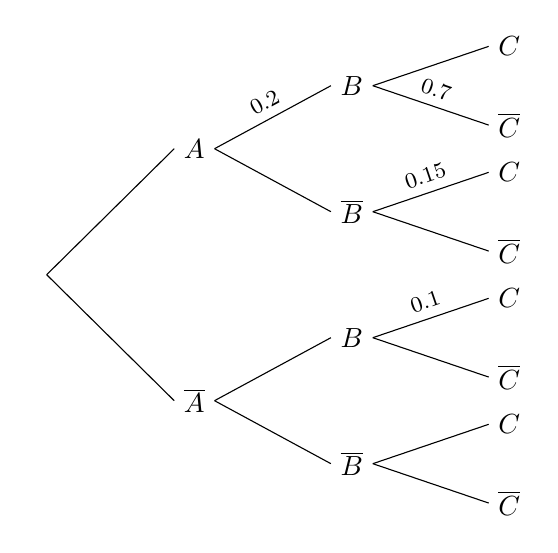
\begin{tikzpicture}[
grow=right,
sloped,
level 1/.style ={level distance=2cm, sibling distance=3.2cm, parent anchor=east, child anchor=west},
level 2/.style ={level distance=2cm, sibling distance=1.6cm},
level 3/.style ={level distance=2cm, sibling distance=1cm},
prob/.style={font=\footnotesize,above}
]

\node (root) {}
child {node {$\overline A$}
child {node {$\overline B$}
child {node {$\overline C$}
}
child {node {$C$}}
}
child {node {$B$}
child {node {$\overline C$}}
child {node {$C$}  edge from parent node[prob] {$0.1$}}
}
}
child {node {$A$}
child {node {$\overline B$}
child {node {$\overline C$}}
child {node {$C$} edge from parent node[prob] {$0.15$}}
}
child {node {$B$}
child {node {$\overline C$}  edge from parent node[prob] {$0.7$}}
child {node {$C$}}
edge from parent node[prob] {$0.2$}
}
};
\end{tikzpicture}
\end{center}

Sabiendo que el $1.5$\% de la población ha tenido las tres enfermedades, que el 54\% no ha tenido ninguna, y que las enfermedades $A$ y $B$ son independientes, se pide:

\begin{enumerate}
\item Completar el árbol etiquetando las ramas con las probabilidades correspondientes.
\item Calcular la probabilidad de tener la enfermedad $C$.
\item Calcular la probabilidad de tener la enfermedad $B$ si se tiene la enfermedad $C$.
\item Calcular la probabilidad de no tener la enfermedad $A$ si no se tienen las otras dos.
\item ¿Son independientes los sucesos $B$ y $C$?
\end{enumerate}
}
%SOLUCIÓN
{
\begin{enumerate}
\item \hfill\break

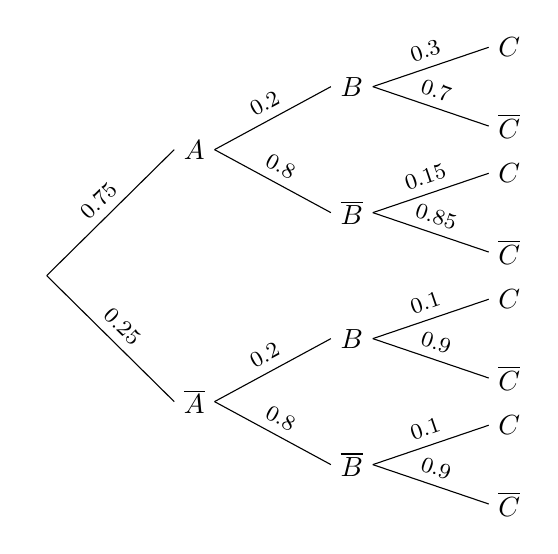
\begin{tikzpicture}[
grow=right,
sloped,
level 1/.style ={level distance=2cm, sibling distance=3.2cm, parent anchor=east, child anchor=west},
level 2/.style ={level distance=2cm, sibling distance=1.6cm},
level 3/.style ={level distance=2cm, sibling distance=1cm},
prob/.style={font=\footnotesize,above}
]

\node (root) {}
child {node {$\overline A$}
child {node {$\overline B$}
child {node {$\overline C$} edge from parent node[prob] {$0.9$}}
child {node {$C$} edge from parent node[prob] {$0.1$}}
edge from parent node[prob] {$0.8$}
}
child {node {$B$}
child {node {$\overline C$} edge from parent node[prob] {$0.9$}}
child {node {$C$}  edge from parent node[prob] {$0.1$}}
edge from parent node[prob] {$0.2$}
}
edge from parent node[prob] {$0.25$}
}
child {node {$A$}
child {node {$\overline B$}
child {node {$\overline C$} edge from parent node[prob] {$0.85$}}
child {node {$C$} edge from parent node[prob] {$0.15$}}
edge from parent node[prob] {$0.8$}
}
child {node {$B$}
child {node {$\overline C$} edge from parent node[prob] {$0.7$}}
child {node {$C$ } edge from parent node[prob] {$0.3$}}
edge from parent node[prob] {$0.2$}
}
edge from parent node[prob] {$0.75$}
};
\end{tikzpicture}

\item $P(C)=0.12$.
\item $P(B|C)=0.25$.
\item $P(\overline A | \overline B \cap \overline C)=0.7606$.
\item No, porque $P(B|C)\neq P(B)$.
\end{enumerate}
}
%RESOLUCIÓN
{
}
